\documentclass{article}
\usepackage[T1]{fontenc}
\usepackage{lmodern}
\usepackage{graphicx}
\usepackage{amsmath,amssymb}
\usepackage[a4paper,margin=2cm]{geometry}
\usepackage[absolute,overlay]{textpos}
\setlength{\TPHorizModule}{1mm}
\setlength{\TPVertModule}{1mm}
\usepackage[indonesian]{babel}
\usepackage{hyperref}
\setlength{\emergencystretch}{2em}
% unit: Halaman 6

\begin{document}

% === Halaman 6 (llm) ===

\vspace{209.98mm}

\begin{equation*}
  y^2 = x^3 - 12x + 13
\end{equation*}

\vspace{10mm}

Sumber gambar: Kevin Tirtawinata, Studi dan Analisis Elliptic Curve Cryptography

% deskripsi: Grafik kurva eliptik berdasarkan persamaan y^2 = x^3 - 12x + 13 pada bidang koordinat Kartesius.
% bbox normalisasi: [0.2850, 0.1130, 0.6600, 0.8200]
\begin{textblock*}{78.75mm}(59.85mm,33.56mm)
\noindent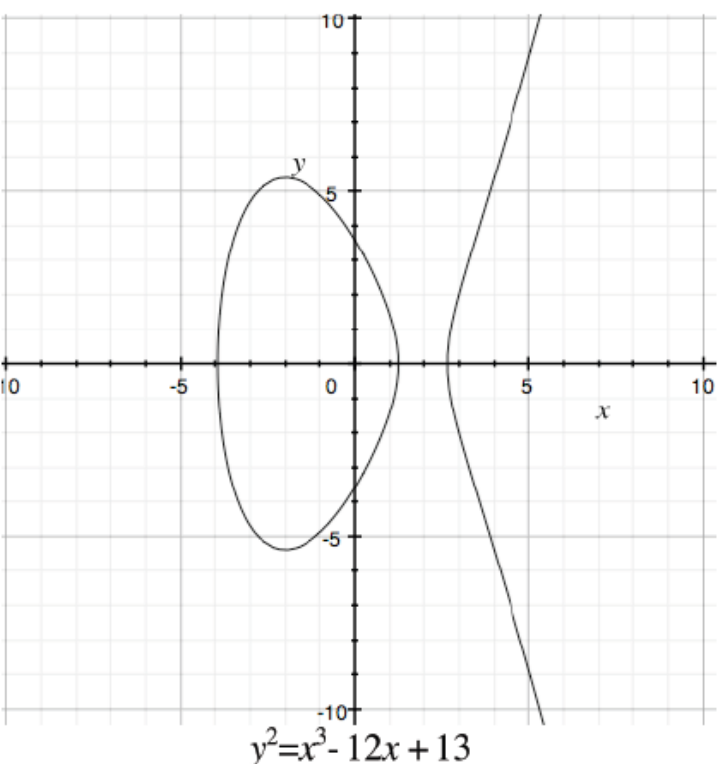
\includegraphics[width=78.75mm,height=209.98mm]{../../images/llm/page_006_img_01.png}%
\end{textblock*}

\end{document}
